\documentclass[main.tex]{subfiles}
\begin{document}

\chapter{The Bootstrap and Resampling Methods}\label{ch:bootstrap}

In earlier chapters we obtained the sampling distribution of an estimator in one of two ways: either exactly (pivots\index{pivot@pivot}, normal sampling theory) or asymptotically (CLT\index{central limit theorem clt@central limit theorem (CLT)}, the delta method\index{delta method@delta method}, Fisher information\index{fisher information@Fisher information}). In many realistic situations, however, both are hard: for the standard error of the median, of a correlation coefficient or of a complicated ratio, there is either no formula or the formula depends on unknown density values. Efron's \cite{efron79} bootstrap\index{bootstrap@bootstrap} solves this problem by computation: it replaces the unknown $F$ by the empirical distribution $\hat F_n$ and simulates the distribution of the estimator by resampling from $\hat F_n$. In this chapter we discuss the plug-in\index{plug in principle@plug-in principle} principle, the bootstrap standard error and bias estimate, four bootstrap confidence intervals, why the bootstrap works (and when it does not), the jackknife\index{jackknife@jackknife} and permutation tests\index{permutation test@permutation test}.

\section{Definitions}

\begin{definition}[Statistical Functional and the Plug-In Principle]\label{def:eklenti}
Write the parameter as a functional of the distribution: $\theta=T(F)$. For example the mean is $T(F)=\int x\,dF(x)$, the median $T(F)=F^{-1}(1/2)$, the variance $T(F)=\int(x-\int y\,dF)^2dF(x)$. The \emph{plug-in\index{plug in principle@plug-in principle} estimator} is obtained by putting the empirical distribution $\hat F_n$ (the discrete distribution giving mass $1/n$ to each observation; Chapter~\ref{ch:rastgele-degiskenler}) in place of $F$: $\hat\theta=T(\hat F_n)$. For example, the plug-in estimator of the variance is $\hat\sigma^2=\frac1n\sum(X_i-\bar X)^2$.
\end{definition}

\begin{definition}[Bootstrap Sample and Bootstrap Distribution]\index{bootstrap@bootstrap|textbf}
After $\x=(x_1,\dots,x_n)$ has been observed, an i.i.d.\ sample of size $n$ from $\hat F_n$ (i.e.\ $n$ draws \emph{with replacement} from $\x$) is called a \emph{bootstrap sample}: $\X^*=(X_1^*,\dots,X_n^*)$. The (conditional) distribution of $\hat\theta^*=T(\hat F_n^*)$ with $\x$ held fixed is called the \emph{bootstrap distribution}; probabilities and expectations under it are denoted $\P^*$ and $\E^*$.
\end{definition}

\begin{definition}[Bootstrap Standard Error and Bias Estimate]\index{bootstrap@bootstrap|textbf}
\[
\widehat{\mathrm{se}}_{\text{boot}}=\sqrt{\Var^*(\hat\theta^*)},\qquad\widehat{\Bias}_{\text{boot}}=\E^*[\hat\theta^*]-\hat\theta .
\]
In practice $B$ bootstrap samples are generated and the sample standard deviation and mean of $\hat\theta^*_1,\dots,\hat\theta^*_B$ are used (a Monte Carlo approximation).
\end{definition}

\begin{definition}[Parametric Bootstrap]\index{bootstrap@bootstrap|textbf}
If the model $\{F_\theta\}$ is known, resampling from $F_{\hat\theta}$ (e.g.\ the distribution estimated by the MLE) instead of $\hat F_n$ is called the \emph{parametric bootstrap\index{bootstrap@bootstrap!parametric@parametric}}.
\end{definition}

\begin{definition}[Bootstrap Confidence Intervals]\label{def:boot-ci}\index{bootstrap@bootstrap|textbf}
Let $\hat\theta^*_{(\alpha)}$ be the $\alpha$ quantile of the bootstrap distribution.
\begin{enumerate}
  \item \textbf{Percentile\index{bootstrap@bootstrap!percentile interval@percentile interval}:} $\big[\hat\theta^*_{(\alpha/2)},\ \hat\theta^*_{(1-\alpha/2)}\big]$.
  \item \textbf{Basic (reverse percentile):} $\big[2\hat\theta-\hat\theta^*_{(1-\alpha/2)},\ 2\hat\theta-\hat\theta^*_{(\alpha/2)}\big]$; it approximates the distribution of $\hat\theta-\theta$ by that of $\hat\theta^*-\hat\theta$.
  \item \textbf{Bootstrap-$t$ (studentised):} with the quantiles $t^*_{(\alpha)}$ of the statistic $t^*=(\hat\theta^*-\hat\theta)/\widehat{\mathrm{se}}^*$, $\big[\hat\theta-t^*_{(1-\alpha/2)}\widehat{\mathrm{se}},\ \hat\theta-t^*_{(\alpha/2)}\widehat{\mathrm{se}}\big]$.
  \item \textbf{BCa\index{bootstrap@bootstrap!bca interval@BCa interval} (bias-corrected and accelerated):} with $\hat z_0=\Phi^{-1}\big(\P^*(\hat\theta^*<\hat\theta)\big)$ and the acceleration $\hat a$ computed from the jackknife values, the endpoints of the percentile interval are shifted to the levels $\alpha_1=\Phi\Big(\hat z_0+\frac{\hat z_0+z_{(\alpha/2)}}{1-\hat a(\hat z_0+z_{(\alpha/2)})}\Big)$ and $\alpha_2$ (similarly, with $z_{(1-\alpha/2)}$): $\big[\hat\theta^*_{(\alpha_1)},\hat\theta^*_{(\alpha_2)}\big]$. Here $z_{(p)}=\Phi^{-1}(p)$.
\end{enumerate}
\end{definition}

\begin{definition}[Jackknife]\label{def:jackknife-tanim}\index{jackknife@jackknife|textbf}
Let $\hat\theta_{(i)}$ be the estimate computed with the $i$-th observation deleted, and $\hat\theta_{(\cdot)}=\frac1n\sum_i\hat\theta_{(i)}$. The jackknife bias and standard error estimates are
\[
\widehat{\Bias}_{\text{jack}}=(n-1)\big(\hat\theta_{(\cdot)}-\hat\theta\big),\qquad
\widehat{\mathrm{se}}_{\text{jack}}=\sqrt{\frac{n-1}{n}\sum_{i=1}^n\big(\hat\theta_{(i)}-\hat\theta_{(\cdot)}\big)^2},
\]
and the bias-corrected estimator is $\hat\theta_{\text{jack}}=\hat\theta-\widehat{\Bias}_{\text{jack}}=n\hat\theta-(n-1)\hat\theta_{(\cdot)}$.
\end{definition}

\begin{definition}[Permutation Test]
For two samples $X_1,\dots,X_m$ and $Y_1,\dots,Y_n$, let $H_0:F_X=F_Y$. The distribution of the values of a statistic $T$ computed over all reassignments of the $N=m+n$ observations into the $\binom Nm$ different groupings is called the \emph{permutation distribution}, and the upper-tail proportion of the observed $T$ in this distribution is the \emph{permutation $p$-value}.
\end{definition}

% <<fig:bootstrap-sema>>
The main idea of the bootstrap is summarised in Figure~\ref{fig:bootstrap-sema}.

\begin{figure}[ht]
\centering
\begin{tikzpicture}[font=\small,
  box/.style={draw,rounded corners=3pt,fill=blue!5,align=center,minimum height=9mm,inner sep=3pt},
  arr/.style={-{Latex[length=2.4mm]},thick}]
\node[font=\bfseries] at (-1.6,1.3) {Real world};
\node[box] (F) at (0,0) {$F$\\\footnotesize unknown};
\node[box] (x) at (3.4,0) {$\x=(x_1,\dots,x_n)$\\\footnotesize one sample};
\node[box] (t) at (7.0,0) {$\hat\theta=T(\x)$\\\footnotesize distribution unknown};
\draw[arr] (F) -- (x); \draw[arr] (x) -- (t);
\node[font=\bfseries] at (-1.4,-1.6) {Bootstrap world};
\node[box,fill=orange!10] (Fh) at (0,-3.2) {$\hat F_n$};
\node[box,fill=orange!10] (x1) at (3.4,-2.3) {$\x^*_1$};
\node at (3.4,-3.2) {$\vdots$};
\node[box,fill=orange!10] (xB) at (3.4,-4.1) {$\x^*_B$};
\node[box,fill=orange!10] (t1) at (6.0,-2.3) {$\hat\theta^*_1$};
\node at (6.0,-3.2) {$\vdots$};
\node[box,fill=orange!10] (tB) at (6.0,-4.1) {$\hat\theta^*_B$};
\draw[arr] (Fh) -- (x1); \draw[arr] (Fh) -- node[below left,font=\footnotesize] {resampling} (xB);
\draw[arr] (x1) -- (t1); \draw[arr] (xB) -- (tB);
\draw[arr,dashed] (x.south) to[bend right=15] (Fh.north);
\begin{scope}[shift={(8.0,-4.3)}]
  \foreach \h [count=\i] in {0.3,0.7,1.2,1.6,1.3,0.8,0.4} \fill[orange!60] (0.25*\i,0) rectangle +(0.22,\h);
  \node[font=\footnotesize,align=center,text width=2.4cm] at (1.0,2.05) {distribution of the $\hat\theta^*$};
\end{scope}
\draw[arr] (t1.east) -- (8.1,-2.5); \draw[arr] (tB.east) -- (8.1,-4.0);
\end{tikzpicture}
\caption{The two worlds of the bootstrap. In the real world a single sample is observed from the unknown $F$, and the sampling distribution of $\hat\theta$ is unknown. In the bootstrap world the empirical distribution $\hat F_n$ takes the place of $F$; since $\hat F_n$ is known, any number of samples ($\x^*_1,\dots,\x^*_B$, drawn from the observations with replacement) can be generated from it, and the distribution of the $\hat\theta^*$ is used in place of the unknown distribution of $\hat\theta$.}\label{fig:bootstrap-sema}
\end{figure}
% <</fig:bootstrap-sema>>

\section{Main Theorems and Proofs}

\begin{proposition}[Structure of a Bootstrap Sample]\label{prop:boot-yapi}\index{bootstrap@bootstrap}
\begin{enumerate}
  \item The probability that a particular $x_i$ does \emph{not} appear at all in a bootstrap sample is $(1-1/n)^n\to e^{-1}\approx0.368$; i.e.\ a bootstrap sample contains on average about $63.2\%$ of the distinct observations.
  \item The number of distinct bootstrap samples, disregarding order, is $\binom{2n-1}{n}$ ($\approx6.9\times10^{10}$ for $n=20$); this is why the bootstrap distribution is in practice approximated by Monte Carlo.
  \item $\E^*[\bar X^*]=\bar x$ and $\Var^*(\bar X^*)=\hat\sigma^2/n$, where $\hat\sigma^2=\frac1n\sum(x_i-\bar x)^2$. Hence the exact bootstrap SE of the mean is $\hat\sigma/\sqrt n$ --- the plug-in\index{plug in principle@plug-in principle} version of the classical formula.
\end{enumerate}
\end{proposition}
\begin{proof}
(1) In each draw the probability that $x_i$ is not selected is $1-1/n$, and the draws are independent. (2) The number of multisets (``stars and bars''): the number of ways of distributing $n$ identical balls into $n$ boxes is $\binom{2n-1}{n}$. (3) The $X_i^*$ are i.i.d.\ from $\hat F_n$, whose mean is $\bar x$ and variance $\hat\sigma^2$.
\end{proof}

\begin{theorem}[Bootstrap Consistency for the Mean \cite{bickel81,singh81}]\label{thm:boot-tutarli}\index{bootstrap@bootstrap}
Let $X_1,X_2,\dots\iid F$ with $\sigma^2=\Var X_1>0$ and $\E|X_1|^3<\infty$. Then, with probability 1,
\[
\sup_{x\in\R}\Big|\P^*\big(\sqrt n(\bar X_n^*-\bar X_n)\le x\big)-\P\big(\sqrt n(\bar X_n-\mu)\le x\big)\Big|\xrightarrow{n\to\infty}0 .
\]
(The result also holds under $\E X_1^2<\infty$ alone \cite{bickel81,singh81}.)
\end{theorem}
\begin{proof}
With the data fixed, the $X_i^*$ are i.i.d.\ variables with mean $\bar X_n$, variance $\hat\sigma_n^2$ and absolute third central moment $\hat\rho_n=\frac1n\sum|X_i-\bar X_n|^3$. Applying the Berry--Esseen\index{berry esseen theorem@Berry--Esseen theorem} theorem (Theorem~\ref{thm:berry-esseen}) to this conditional distribution,
\[
\sup_x\Big|\P^*\Big(\tfrac{\sqrt n(\bar X^*_n-\bar X_n)}{\hat\sigma_n}\le x\Big)-\Phi(x)\Big|\le\frac{C\hat\rho_n}{\hat\sigma_n^3\sqrt n}.
\]
By the SLLN\index{law of large numbers@law of large numbers!strong slln@strong (SLLN)}, $\hat\sigma_n\asto\sigma>0$ and $\hat\rho_n\asto\E|X_1-\mu|^3<\infty$; hence the right-hand side goes to $0$ a.s. On the other hand, by the CLT\index{central limit theorem clt@central limit theorem (CLT)} $\P(\sqrt n(\bar X_n-\mu)/\sigma\le x)\to\Phi(x)$, and since the limit is continuous the convergence is uniform (Pólya). Both distributions converge uniformly to $\Normal(0,\sigma^2)$ and $\hat\sigma_n/\sigma\to1$; the triangle inequality gives the result.
\end{proof}

\begin{remark}[Second-Order Accuracy]
Theorem~\ref{thm:boot-tutarli} says that the bootstrap is at least as good as the normal approximation. More is true: by Edgeworth expansions, for \emph{pivotal\index{pivot@pivot}} (studentised) statistics the error of the bootstrap approximation is $O_P(n^{-1})$, whereas that of the normal approximation is $O(n^{-1/2})$ \cite{hall}. The bootstrap captures the skewness\index{skewness@skewness} term ``automatically''. This is the theoretical reason why the coverage error of bootstrap-$t$ and BCa\index{bootstrap@bootstrap!bca interval@BCa interval} intervals is $O(n^{-1})$, while that of percentile\index{bootstrap@bootstrap!percentile interval@percentile interval} and normal intervals is generally $O(n^{-1/2})$. But this is an asymptotic ranking; the actual performance in finite samples must be checked by simulation (in the coverage table below, BCa falls behind the classical $t$ at $n=20$).
\end{remark}

\begin{theorem}[Jackknife Bias Correction]\label{thm:jackknife}\index{jackknife@jackknife}
If $\E\hat\theta_n=\theta+\frac{a}{n}+\frac{b}{n^2}+O(n^{-3})$ (with the same $a,b$ for all $n$), then the bias of the jackknife estimator is $O(n^{-2})$:
\[
\E\hat\theta_{\text{jack}}=\theta-\frac{b}{n(n-1)}+O(n^{-2}) .
\]
\end{theorem}
\begin{proof}
Since each $\hat\theta_{(i)}$ is based on $n-1$ observations, $\E\hat\theta_{(\cdot)}=\theta+\frac{a}{n-1}+\frac{b}{(n-1)^2}+O(n^{-3})$. Thus
\[
\E\hat\theta_{\text{jack}}=n\Big(\theta+\frac an+\frac b{n^2}\Big)-(n-1)\Big(\theta+\frac a{n-1}+\frac b{(n-1)^2}\Big)+O(n^{-2})=\theta+\frac bn-\frac b{n-1}+O(n^{-2}),
\]
and $\frac bn-\frac b{n-1}=-\frac{b}{n(n-1)}$. The bias of order $1/n$ disappears completely.
\end{proof}

\begin{example}[The Jackknife Turns $\hat\sigma^2$ into $S^2$]
For $\hat\theta=\hat\sigma^2$, $\E\hat\sigma^2=\sigma^2-\sigma^2/n$, i.e.\ $a=-\sigma^2$, $b=0$. Theorem~\ref{thm:jackknife} says that the jackknife estimator is unbiased; direct computation gives $\hat\theta_{\text{jack}}=S^2$ (verified with the code below).
\end{example}

\begin{theorem}[Exact Level of the Permutation Test]\label{thm:permutasyon}
Under $H_0$ let $(Z_1,\dots,Z_N)=(X_1,\dots,X_m,Y_1,\dots,Y_n)$ be exchangeable\index{exchangeability@exchangeability}, i.e.\ every permutation has the same joint distribution (i.i.d.\ with $F_X=F_Y$ ensures this). If $T_0$ is the observed statistic and $T_1,\dots,T_B$ are the values computed from random permutations, then for
\[
p=\frac{1+\#\{b:T_b\ge T_0\}}{B+1}
\]
we have $\P_{H_0}(p\le\alpha)\le\alpha$ for every $\alpha\in(0,1)$. That is, the permutation test\index{permutation test@permutation test} has level exactly $\alpha$ for every $n$, \emph{without any distributional assumption}.
\end{theorem}
\begin{proof}
Under $H_0$, $(T_0,T_1,\dots,T_B)$ is exchangeable: the observed assignment has the same distribution as any of the random assignments. Hence (if there are no ties) the rank of $T_0$ among these $B+1$ values is uniformly distributed on $\{1,\dots,B+1\}$ and $\P(p\le k/(B+1))=k/(B+1)$; with ties the probability is at most this.
\end{proof}

\section{Worked Examples}

\begin{example}[Standard Error of the Median]\label{ex:medyan-se}
The asymptotic standard error of the sample median is $1/(2f(m)\sqrt n)$ (Example~\ref{ex:are}); but $f(m)$ is the value of the unknown density at the median, and estimating it requires choosing a bandwidth\index{bandwidth@bandwidth}. The bootstrap\index{bootstrap@bootstrap} SE requires no density estimate: resample $B$ times, compute the median each time, and take the standard deviation. For Exp(1) data the true values are $m=\ln2$, $f(m)=\frac12$, and the asymptotic SE is $1/\sqrt n$.
\end{example}

\begin{example}[Where the Bootstrap Fails: An Extreme Value]\label{ex:boot-basarisiz}
$X_i\iid\text{Uniform}(0,\theta)$, $\hat\theta=X_{(n)}$. The true distribution: $n(\theta-X_{(n)})/\theta\dto\text{Exp}(1)$, a continuous limit. In the bootstrap, however,
\[
\P^*\big(X^*_{(n)}=X_{(n)}\big)=1-\Big(1-\frac1n\Big)^n\to1-e^{-1}\approx0.632 .
\]
The bootstrap distribution has an atom of $63\%$ at $0$, whereas the true distribution has no atom. The bootstrap is inconsistent. Why: the functional $T(F)=F^{-1}(1)$ is not ``smooth'' (Hadamard differentiable) at $F$, and $\hat F_n$ cannot imitate the upper end of $F$. The parametric bootstrap\index{bootstrap@bootstrap!parametric@parametric} (resampling from $\text{Uniform}(0,X_{(n)})$), on the other hand, works.
\end{example}

\begin{example}[Permutation Test]
Let there be $m$ observations in a treatment group and $n$ in a control group, and $T=\bar Y-\bar X$. The observations are pooled, a random $m$ of them receive the label ``treatment'', and $T$ is recomputed; this is repeated $B$ times. This test is the essence of Fisher's \cite{fisher35} idea of ``randomisation inference'': random assignment is the source of the test's validity; no normality assumption is needed.
\end{example}

\section{Computational Applications}

\subsection{Bootstrap Standard Error of the Median}

\pycode{code/ch18/c18_1_bootstrap_se_of_median.py}
\begin{lstlisting}[style=output]
Observed median = 0.6487 (true ln2 = 0.6931)
Median SE: bootstrap = 0.1955 | true (MC) = 0.1406 | asymptotic 1/sqrt(n) = 0.1414
Mean SE: bootstrap = 0.1009 | plug-in formula sigma_hat/sqrt(n) = 0.1006
Proportion of distinct observations in a bootstrap sample ≈ 0.632 (1-1/e = 0.632)
Number of distinct values in the bootstrap distribution of the median: 121 / 4000
\end{lstlisting}

As predicted by Proposition~\ref{prop:boot-yapi}(3), the bootstrap\index{bootstrap@bootstrap} SE of the mean agrees almost exactly with the plug-in\index{plug in principle@plug-in principle} formula. The bootstrap SE of the median, however, is clearly above the true value ($0.141$) in this sample. This is not a mistake but the unavoidable variability of any estimate made from a single sample: in an additional simulation with $1000$ separate exponential samples, the bootstrap SE of the median had mean $0.146$ (i.e.\ it is approximately unbiased) but standard deviation $0.043$; $90\%$ of the values lay between $0.089$ and $0.231$. The relative variability is larger (about $29\%$) than for the mean (about $20\%$), because the bootstrap distribution of the median rests on a few central observations and is step-like. Lesson: the bootstrap SE is itself an estimate and has its own uncertainty.

\begin{figure}[h]
\centering
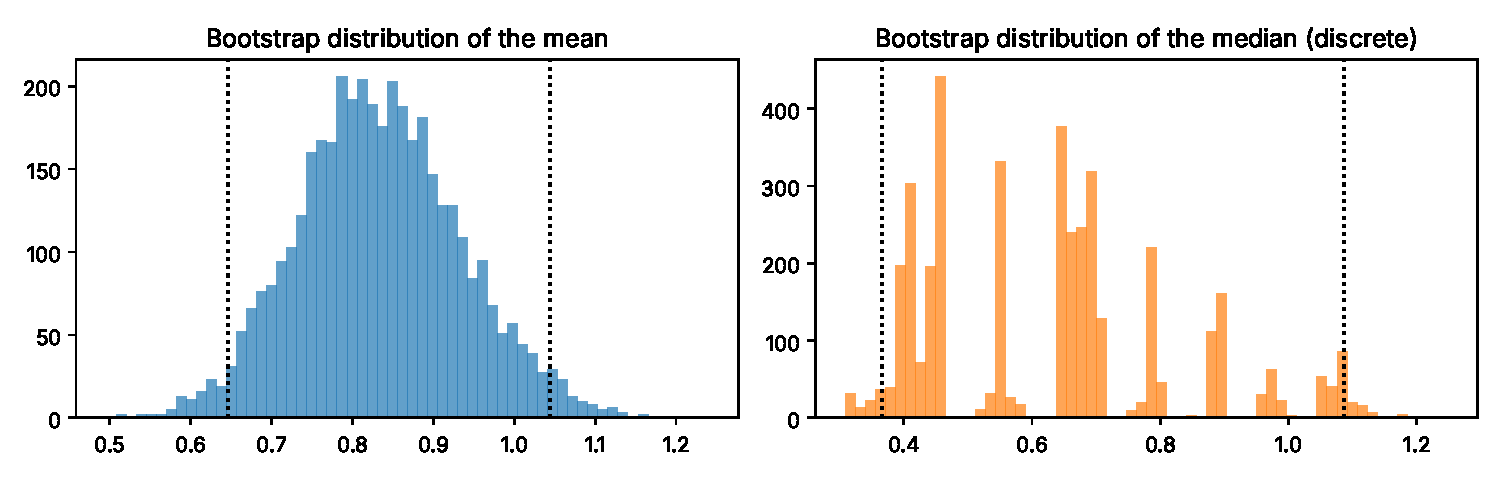
\includegraphics[width=0.95\textwidth]{figures/bootstrap_dagilim.pdf}
\caption{Bootstrap distributions obtained from the same exponential sample ($n=50$); the dotted lines are the endpoints of the $95\%$ percentile interval. Since the median can take only observed values (or the average of two observations), its bootstrap distribution is ``step-like''.}
\end{figure}

\subsection{Coverage of Bootstrap Confidence Intervals}
We generate $M=2000$ data sets of size $n=20$ from the Exp(1) distribution and in each construct five different $95\%$ intervals for $\mu$. The skewed distribution and the small $n$ bring out the differences between the methods.

\pycode{code/ch18/c18_2_coverage_of_bootstrap_intervals.py}
\begin{lstlisting}[style=output]
Method       | coverage | interval left of mu | mean length
t (classic)  |  0.9250  |       0.0685        |   0.9032
Percentile   |  0.9060  |       0.0760        |   0.8157
Basic        |  0.8890  |       0.1000        |   0.8157
Bootstrap-t  |  0.9385  |       0.0410        |   1.0531
BCa          |  0.9115  |       0.0570        |   0.8623
\end{lstlisting}

For skewed data the classical $t$, percentile\index{bootstrap@bootstrap!percentile interval@percentile interval} and basic intervals stay below the nominal level, and their errors are asymmetric: when they miss, the interval usually lies to the \emph{left} of $\mu$ (since large observations in the right tail are rare, in small samples $\bar X$ is usually below $\mu$). The percentile and basic intervals are even worse than the classical $t$: they are scaled by $\hat\sigma$ (with divisor $1/n$) and do not include the small-sample widening of the $t$ quantiles. BCa\index{bootstrap@bootstrap!bca interval@BCa interval} improves the percentile interval with a bias and skewness\index{skewness@skewness} correction, but at $n=20$ it still falls behind the classical $t$; the acceleration $\hat a$ is itself a noisy estimate in small samples. The method that comes closest to the nominal level and has the most balanced errors is the \emph{bootstrap-$t$}; the price is noticeably longer intervals, asymmetric to the right. This is the numerical counterpart of the second-order accuracy that arises when bootstrapping pivotal\index{pivot@pivot} statistics. Lesson: saying ``I used the bootstrap'' is no guarantee on its own; in small samples, which interval is used is decisive.

\subsection{Failure: The Maximum of $\text{Uniform}(0,\theta)$}

\pycode{code/ch18/c18_3_failure_uniform_maximum.py}
\begin{lstlisting}[style=output]
P*(X*_(n) = X_(n)) = 0.6410 | theory 1-(1-1/n)^n = 0.6358
True distribution    | n(theta-max)/theta: P(=0)=0.000 | quartiles=[0.284 0.678 1.346] (Exp(1): [0.288 0.693 1.386])
Nonparametric        | n(theta-max)/theta: P(=0)=0.641 | quartiles=[0.    0.    0.252] (Exp(1): [0.288 0.693 1.386])
Parametric bootstrap | n(theta-max)/theta: P(=0)=0.000 | quartiles=[0.289 0.688 1.381] (Exp(1): [0.288 0.693 1.386])
\end{lstlisting}

\subsection{Jackknife and Permutation Test}

\pycode{code/ch18/c18_4_jackknife_permutation_test.py}
\begin{lstlisting}[style=output]
sigma_hat^2 = 3.15749 | jackknife-corrected = 3.38303 | S^2 = 3.38303
Number of distinct median jackknife values: 3 (n=15) -> SE estimate unreliable
Permutation p = 0.0119 | Welch t-test p = 0.0841
rejection rate under H0 (target 0.05): permutation = 0.057 | Welch t = 0.026
\end{lstlisting}

Three observations: (i) The jackknife\index{jackknife@jackknife} correction turns $\hat\sigma^2$ exactly into $S^2$ (Theorem~\ref{thm:jackknife}, $b=0$). (ii) When a single observation is deleted, the median takes only a few distinct values; the jackknife SE is therefore inconsistent for non-smooth statistics such as the median (the bootstrap is consistent). (iii) Under $H_0$, in small and skewed samples, the permutation test\index{permutation test@permutation test} keeps its exact level (Theorem~\ref{thm:permutasyon}) while the Welch\index{welch approximation@Welch approximation} $t$-test is overly conservative; this is why the permutation test can be more powerful on the same data.

\subsection{Real Data: Law Schools and the Bootstrap of a Correlation}\label{sec:hukuk}
The data Efron and Tibshirani used to introduce the bootstrap \cite{efron-tib}: the average LSAT score and undergraduate GPA of 82 US law schools, and a random sample of 15 schools from this population. These data offer a rare situation: since the population is known, the \emph{true} sampling distribution that the bootstrap tries to approximate can also be computed. The code computes the bootstrap standard error of the sample correlation $r$ and four $95\%$ intervals: percentile, basic, BCa, and the Fisher $z$ interval based on bivariate normality (Example~\ref{ex:varyans-dengeleme}). It then draws 15 schools from the population without replacement to find the true standard deviation of $r$.

\pycode{code/ch18/c18_5_law_schools_real_data.py}
\begin{lstlisting}[style=output]
sample r = 0.7764 | bootstrap SE = 0.1354, bias = -0.0058
95% intervals: percentile [0.456, 0.962] | basic [0.591, 1.097] | BCa [0.317, 0.943] | Fisher z [0.439, 0.922]
BCa constants: z0 = -0.105, acceleration a = -0.076
population rho = 0.7600 | true SD(r) = 0.1185 | E(r) = 0.7486
\end{lstlisting}

The bootstrap standard error ($0.135$) is somewhat above the true value ($0.119$). Part of the difference is that the bootstrap draws from 15 observations \emph{with} replacement, whereas the actual sample was drawn from 82 schools \emph{without} replacement. Multiplied by the finite-population correction $\sqrt{(82-15)/(82-1)}\approx0.91$, the bootstrap SE is $\approx0.123$, closer to the true value. The behaviour of the intervals is instructive. The bootstrap distribution of $r$ is skewed to the left. The \emph{basic} interval reflects this skewness in the wrong direction, so its upper end is $1.097$, outside the possible values of a correlation. The percentile and BCa intervals respect transformations and stay inside $[-1,1]$. The BCa interval extends further to the left because of its skewness ($a<0$) and bias ($z_0<0$) corrections. The normal-theory Fisher $z$ interval is close to the percentile interval. The population correlation $\rho=0.760$ lies inside all four intervals.

\section{Comments and Notes}

\begin{remark}[When Does the Bootstrap Work?]
The general principle: if $\sqrt n(T(\hat F_n)-T(F))$ has a normal limit and $T$ is ``smooth'' (Hadamard differentiable) near $F$, the bootstrap\index{bootstrap@bootstrap} is consistent. This covers smooth functionals such as means, moments, quantiles (if the density is positive), the correlation, regression coefficients and the MLE. Typical situations where it fails: extreme values (Example~\ref{ex:boot-basarisiz}), the boundary of the parameter space, heavy tails with infinite variance (in which case the ``$m$-out-of-$n$'' bootstrap with resamples of size $m<n$ is used), and dependent data (the block bootstrap is needed).
\end{remark}

\begin{remark}[How Many Bootstrap Samples?]
For estimating an SE, $B\approx200$--$1000$ is usually enough; the Monte Carlo error stays small next to the bootstrap's own sampling error. Since the endpoints of confidence intervals rest on tail quantiles, $B\ge2000$ is recommended for them, and for $p$-values $B+1$ should be chosen compatibly with $\alpha$ (e.g.\ $B=999$).
\end{remark}

\begin{remark}[The Bootstrap and Bayes]
The bootstrap distribution is very tempting to read as a probability distribution over $\theta$. Rubin's \cite{rubin81} \emph{Bayesian bootstrap} makes this intuition precise: if the observation weights are drawn from $\text{Dirichlet}(1,\dots,1)$, the resulting distribution is the posterior under a non-informative Dirichlet process prior. The classical bootstrap draws the weights from $\text{Multinom}(n;1/n,\dots,1/n)/n$; the two distributions agree to first order (compare with Bernstein--von Mises\index{bernstein von mises theorem@Bernstein--von Mises theorem} in Chapter~\ref{ch:bayes}).
\end{remark}

\begin{remark}[Permutation or Bootstrap?]
Permutation tests\index{permutation test@permutation test} give an \emph{exact} level when exchangeability\index{exchangeability@exchangeability} holds under $H_0$, but they test only sharp hypotheses such as ``the distributions are equal''. Bootstrap tests are more flexible (e.g.\ equality of means only, with different variances), but their level is only asymptotically correct. A frequently forgotten point is that in a bootstrap hypothesis test the resampling must be done so as to satisfy $H_0$ (e.g.\ by shifting the groups to a common mean).
\end{remark}

% --- CHAPTER SUMMARY ---
\section{Chapter Summary}
\begin{summary}
\begin{itemize}
  \item By the plug-in principle, the unknown $F$ is replaced by the empirical distribution $\hat F_n$ (Definition~\ref{def:eklenti}). The bootstrap approximates the sampling distribution of a statistic by resampling from $\hat F_n$.
  \item The bootstrap gives standard error and bias estimates. The types of confidence interval are percentile, basic, studentised and BCa (Definition~\ref{def:boot-ci}).
  \item For smooth statistics such as the mean the bootstrap is consistent (Theorem~\ref{thm:boot-tutarli}). It fails for irregular statistics such as the sample maximum.
  \item The jackknife reduces the bias from $O(1/n)$ to $O(1/n^2)$ (Theorem~\ref{thm:jackknife}). The permutation test has exact level under exchangeability (Theorem~\ref{thm:permutasyon}).
  \item The bootstrap is no miracle. In small samples $\hat F_n$ cannot represent the tails well, and intervals may have low coverage.
\end{itemize}
\end{summary}
% --- END OF CHAPTER SUMMARY ---

\paragraph{Further reading.} \cite{efron-tib}, \cite{davison}; for the theoretical foundations, \cite{hall} and \cite[Chapter~23]{vdv}.

\section{Exercises}

\begin{exercise}\label{exr:18-1}
Repeat the Fisher $z$ exercise of Chapter~\ref{ch:mle-asimptotik}: for bivariate normal data ($\rho=0.8$, $n=20$), compare the coverage of the percentile, BCa and Fisher $z$ intervals for the correlation coefficient. How does the result change if the data are not normal (e.g.\ bivariate lognormal)?
\hfill\hyperref[coz:18-1]{\footnotesize$\rightarrow$\,Solution}
\end{exercise}

\begin{exercise}\label{exr:18-2}
In linear regression (Chapter~\ref{ch:dogrusal}), apply the \emph{case} (pairs) bootstrap and the \emph{residual} bootstrap. If the error variance changes with the explanatory variable (heteroscedasticity), which gives a valid standard error? Compare the result with the sandwich estimator of Proposition~\ref{prop:sandvic}. Show this by simulation.
\hfill\hyperref[coz:18-2]{\footnotesize$\rightarrow$\,Solution}
\end{exercise}

\begin{exercise}\label{exr:18-3}
For $X_i\iid\text{Cauchy}(\theta,1)$ data, compute the bootstrap SE of the sample mean repeatedly with $B=1000$. Relate the instability of the results to the Cauchy example of Chapter~\ref{ch:esitsizlikler}. What happens for the median?
\hfill\hyperref[coz:18-3]{\footnotesize$\rightarrow$\,Solution}
\end{exercise}

\begin{exercise}\label{exr:18-4}
Using Theorem~\ref{thm:jackknife}, show that the jackknife-corrected version of $\hat\theta=\bar X^2$ (an estimate of $\mu^2$) is exactly unbiased, and compare the result with $\bar X^2-S^2/n$.
\hfill\hyperref[coz:18-4]{\footnotesize$\rightarrow$\,Solution}
\end{exercise}

\begin{exercise}\label{exr:18-5}
For the law-school sample (Section~\ref{sec:hukuk}), compute the jackknife standard error of $r$ (Definition~\ref{def:jackknife-tanim}) and compare it with the bootstrap SE and with the true SD found from the population. For what kind of statistics is the jackknife unreliable?
\hfill\hyperref[coz:18-5]{\footnotesize$\rightarrow$\,Solution}
\end{exercise}

\chapterlinks{18}

\end{document}
